\begin{figure}[b]
    \centering
    \begin{subfigure}[t]{0.3\textwidth}
    \centering
        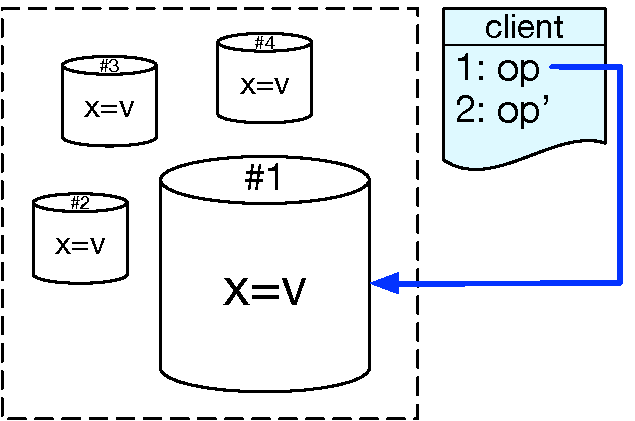
\includegraphics[scale=0.32]{Figures/system_model1.pdf}
        \subcaption{\scriptsize A client submits an operation $\op$ to the store, which
	is routed to the replica \texttt{\#1}.}
        \label{fig:sys_model1}
    \end{subfigure}
    \hfill
    \vline
    \hfill
    \begin{subfigure}[t]{0.3\textwidth}
        \centering
	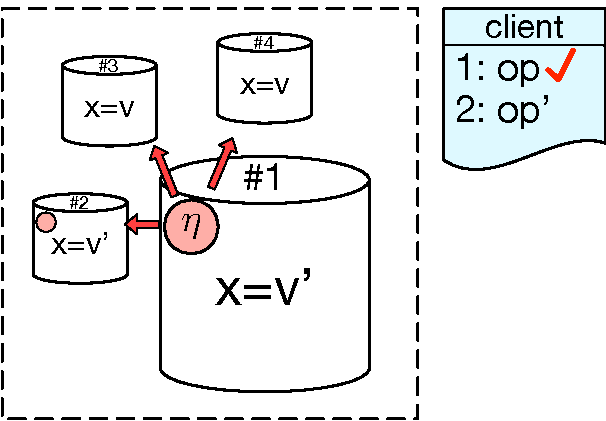
\includegraphics[scale=0.32]{Figures/system_model2.pdf}
        \subcaption{\scriptsize The state of the replica \texttt{\#1} is updated, an
	effect is created and is being propagated}
        \label{fig:sys_model2}
    \end{subfigure}
    \hfill
    \vline
    \hfill
    \begin{subfigure}[t]{0.3\textwidth}
        \centering
	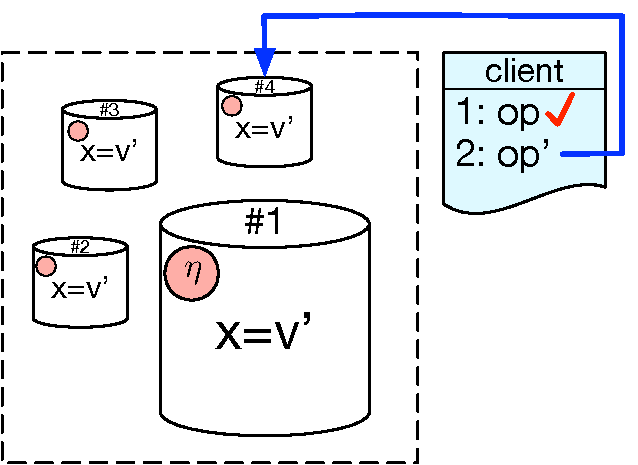
\includegraphics[scale=0.32]{Figures/system_model3.pdf}
        \subcaption{\scriptsize Second operation $\op'$ is submitted to the store, which
	is routed to the replica \texttt{\#4}}
        \label{fig:sys_model3}
    \end{subfigure}
    \caption{system model of \tool}\label{fig:system_model}
\end{figure}
